% 자동 생성: scripts/plot_nparty_dist.py — 수정은 스크립트에서
% 데이터: nparty-tracks-20260814T001421Z cases.jsonl (functional-ext2 정본 — 전 480케이스/방안 (결렬 포함, 24 §4 모수))
\documentclass[tikz,border=2pt]{standalone}
\usepackage{pgfplots}
\pgfplotsset{compat=1.18}
\definecolor{planblue}{HTML}{3A6FE0}
\definecolor{planred}{HTML}{D5484A}
\begin{document}
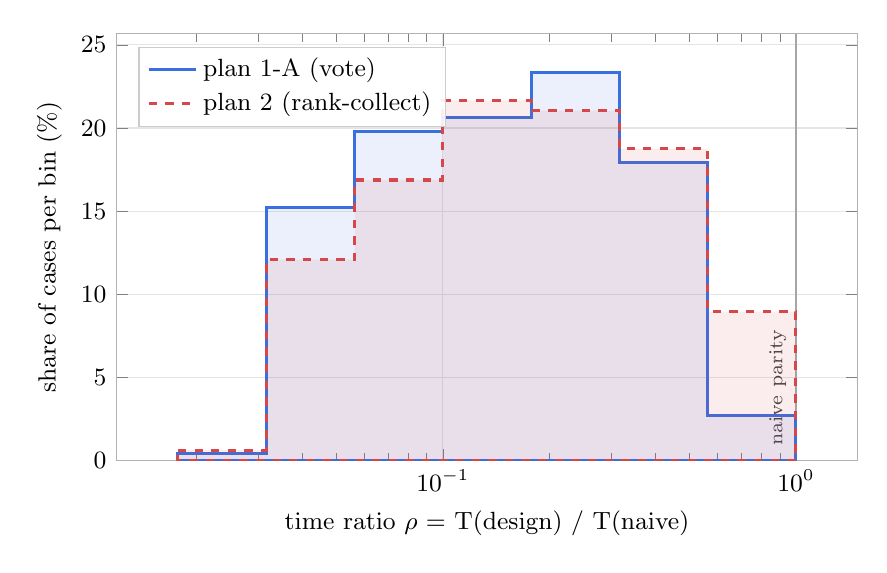
\begin{tikzpicture}
\begin{axis}[
  width=11cm, height=7cm,
  xmode=log,
  xlabel={time ratio $\rho$ = T(design) / T(naive)},
  ylabel={share of cases per bin (\%)},
  ymin=0,
  grid=major, grid style={gray!20},
  axis line style={gray!60},
  tick label style={font=\small},
  label style={font=\small},
  legend style={at={(0.03,0.97)}, anchor=north west, font=\small,
                 draw=gray!40, fill=white, fill opacity=0.9, text opacity=1},
  legend cell align=left,
]
\draw[gray!70, thin] (axis cs:1,0) -- (axis cs:1,\pgfkeysvalueof{/pgfplots/ymax});
\node[gray!50!black, font=\scriptsize, anchor=south west, rotate=90]
  at (axis cs:1,0.3) {naive parity};
\addplot[planblue, solid, line width=1.1pt, const plot,
  fill=planblue, fill opacity=0.10, draw opacity=1] coordinates {
(0.0177828,0.417)(0.0316228,15.208)(0.0562341,19.792)(0.1,20.625)(0.177828,23.333)
(0.316228,17.917)(0.562341,2.708)(1,2.708)} \closedcycle;
\addlegendentry{plan 1-A (vote)}
\addplot[planred, dashed, line width=1.1pt, const plot,
  fill=planred, fill opacity=0.10, draw opacity=1] coordinates {
(0.0177828,0.625)(0.0316228,12.083)(0.0562341,16.875)(0.1,21.667)(0.177828,21.042)
(0.316228,18.750)(0.562341,8.958)(1,8.958)} \closedcycle;
\addlegendentry{plan 2 (rank-collect)}
\end{axis}
\end{tikzpicture}
\end{document}
